\documentclass[12pt,a4paper]{ctexart}

\usepackage[UTF8]{ctex}
\usepackage{geometry}
\usepackage{graphicx}
\usepackage{xcolor}
\usepackage{tikz}
\usepackage{fontspec}
\usepackage{setspace}
\usepackage{enumitem}
\usepackage{booktabs}
\usepackage{array}
\usepackage{longtable}
\usepackage{hyperref}
\usepackage{fancyhdr}
\usepackage{titlesec}
\usepackage{multicol}
\usepackage{xurl}
\usepackage{tocloft}

\renewcommand{\cfttoctitlefont}{\hfill\bfseries\Large}
\renewcommand{\cftaftertoctitle}{\hfill}
\geometry{left=2.5cm,right=2.5cm,top=2.5cm,bottom=2.5cm}

\definecolor{black}{RGB}{0,0,0}
\definecolor{mainblue}{RGB}{0,82,147}
\definecolor{accentgold}{RGB}{180,140,60}
\definecolor{lightgray}{RGB}{245,245,245}
\definecolor{darkgray}{RGB}{80,80,80}
\definecolor{mainred}{RGB}{230,1,45}

\hypersetup{
    colorlinks=true,
    linkcolor=black,
    urlcolor=mainblue,
    citecolor=mainblue,
    pdfborder={0 0 0}
}

\pagestyle{fancy}
\fancyhf{}
\fancyhead[L]{\small\color{darkgray}\textbf{量子行业每周新闻洞察}}
\fancyhead[R]{\small\color{darkgray}\textbf{总第188期}}
\fancyfoot[C]{\thepage}
\renewcommand{\headrulewidth}{0.4pt}
\renewcommand{\footrulewidth}{0pt}

\titleformat{\section}
    {\Large\bfseries\color{mainred}}
    {\thesection、}{0em}{}
\titleformat{\subsection}
    {\large\bfseries\color{mainred}}
    {\thesubsection、}{0em}{}

\newcolumntype{L}[1]{>{\raggedright\arraybackslash}p{#1}}
\newcolumntype{C}[1]{>{\centering\arraybackslash}p{#1}}

\begin{document}

% ==================== 封面 ====================
\begin{titlepage}
\begin{tikzpicture}[remember picture,overlay]
    \fill[mainred] ([yshift=-0.5cm]current page.north west) rectangle ([yshift=-1.2cm]current page.north east);
    \fill[mainred] ([yshift=1.2cm]current page.south west) rectangle ([yshift=0.5cm]current page.south east);
\end{tikzpicture}

\vspace*{4cm}

\begin{center}
    {\fontsize{44}{52}\selectfont\bfseries\color{black} \textbf{量子行业每周新闻洞察}}

    \vspace{0.8cm}

    {\fontsize{16}{22}\selectfont\color{darkgray} 2026.07.11 — 2026.07.17 }
    {\fontsize{16}{22}\selectfont\color{darkgray} \textbf{WEEKLY NEWS}}

    \vspace{1.5cm}

    {\fontsize{20}{26}\selectfont\color{mainred}\textbf{（总第\textbf{ 188 }期）}}

    \vspace{4cm}

    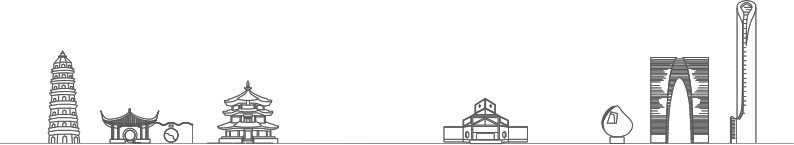
\includegraphics[width=\textwidth]{Cover_Suzhou.png}

    \vfill

    {\fontsize{12}{16}\selectfont\color{darkgray} 量子科技长三角产业创新中心\\编制：战略情报与成果专利室、产业发展部（理事会办公室）}
\end{center}
\end{titlepage}

% ==================== 目录 ====================
\pagenumbering{roman}
\newpage
\tableofcontents

\newpage

% ==================== 摘要 ====================
\pagenumbering{arabic}
\setcounter{page}{1}
\begin{center}
{\Large\bfseries\color{mainred} 摘\hspace{2em}要}
\end{center}
\addcontentsline{toc}{section}{摘要}


\textbf{ 宏观态势：}

全球量子科技竞争正从单一技术突破转向生态体系与全链条战略构建。欧美在量子通信网络建设上加速协同，通过大型联盟与项目推动城域级量子中继器部署及面向工业认证的安全通信技术发展。与此同时，后量子密码与量子安全解决方案的落地步伐加快，企业、资本与科研机构正聚焦于帮助组织平稳过渡至量子安全时代。区域创新生态也在成型，通过加速器项目和区域经济研讨，培育初创企业与跨州合作网络，为构建量子产业高地蓄力。


\textbf{ 科技前沿：}

基础研究与量子计算软硬件实现齐头并进。在量子比特层面，GKP纠错和八量子比特硅基阵列等关键突破，印证了容错量子计算正从理论走向工程验证。量子网络研究在分布式纠缠与量子存储领域取得进展，为实现更高效的信息传递与处理奠定基础。量子材料领域成果斐然，从二维材料精准调控到拓扑光子学与准晶量子几何研究，科学家正利用新方法与新平台，探索新物态并开发高精度测量技术。量子经典融合算法、光量子模拟器等研究亦展现了多路径逼近实用化的趋势。


\textbf{ 产品动态：}

量子技术正从实验室走向专业级产品与特定场景应用。欧洲航天局部署融合经典计算的混合量子计算机，标志着量子计算在航空航天等关键部门的实用化迈出坚实一步。在导航、通信安全与工业仿真领域，适航认证的量子导航系统、量子安全芯片及通用光量子计算架构相继发布或交付，表明特定领域的量子硬件产品正在成熟。同时，量子AI赋能医学影像等跨界应用，以及高端科研仪器交付，显示量子衍生技术也在创造新市场空间。


\textbf{ 企业资讯：}

全球量子企业生态呈现活跃的合作与专业化扩张态势。一方面，跨行业战略合作深化，量子计算公司正与航空航天、工业设计及半导体企业联手，探索具体应用场景，并推进人才联合培养。另一方面，企业正积极进行组织架构优化与全球布局，通过任命商业高管、设立新办公室等方式加速市场化进程。技术应用上，量子安全防护与通信技术集成趋势明显，而专注于超导处理器数字孪生、分布式计算安全控制等细分领域的企业亦在强化其产业链定位。


\textbf{ 资本运作：}

资本对量子技术的支持正向深度产业化聚焦。巨额投资正投向特定技术路线的规模化制造，例如欧洲斥资建设中性原子量子芯片生产线，彰显了从研发到量产的决心。区域性量子创新基金持续拨款扶持初创企业，而企业端的大额融资，特别是结合国家芯片法案的资金注入，为从材料到系统的各环节发展提供了关键动力。值得注意的是，市场迎来首家纯量子计算上市公司，资本退出通道的出现标志着行业开始步入成熟的新阶段。




\textbf{ 专利动态：}

本周专利动态涵盖低温环境系统、超导量子测控技术、量子软件与算法、量子算力网、量子科技长三角产业创新中心共5个板块、19条专利。




% ==================== 会议列表 ====================
{
    \newpage
    \section*{ 7月量子科技行业国内、国际会议}
    \addcontentsline{toc}{section}{ 7月量子科技行业国内、国际会议}
    \scriptsize
    \begin{longtable}{C{0.8cm}L{2.5cm}L{3cm}L{7cm}}
        \toprule[1.5pt]
        \textbf{序号} & \textbf{日期} & \textbf{地点} & \textbf{会议名称} \\
        \midrule
        \endfirsthead
        \toprule
        \textbf{序号} & \textbf{日期} & \textbf{地点} & \textbf{会议名称} \\
        \midrule
        \endhead
        \bottomrule
        \endfoot
        
        1 & 7月1日-3日 & 奥尔堡, 丹麦 & IEEE量子控制、计算与学习国际会议（IEEE qCCL 2026） \\
        \midrule[0.05pt]
        
        2 & 7月1日-3日 & 首尔, 韩国 & 2026量子信息会议（CQI 2026） \\
        \midrule[0.05pt]
        
        3 & 7月1日-3日 & 爱丁堡, 英国 & 2026青年量子研究者暑期学校 \\
        \midrule[0.05pt]
        
        4 & 7月2日-4日 & 首尔, 韩国 & Quantum Korea 2026 \\
        \midrule[0.05pt]
        
        5 & 7月6日-8日 & 海尔布隆, 德国 & 自然科学容错量子计算研讨会（FTQC4NSc） \\
        \midrule[0.05pt]
        
        6 & 7月6日-10日 & 那不勒斯, 意大利 & 第12届单光子研讨会（SPW 2026） \\
        \midrule[0.05pt]
        
        7 & 7月7日-10日 & 加尔各答, 印度 & 2026年IEEE量子计算国际研讨会：电路、系统、自动化与应用（QC-CSAA） \\
        \midrule[0.05pt]
        
        8 & 7月12日-17日 & 马斯特里赫特, 荷兰 & 量子传感与计量学（QSM） \\
        \midrule[0.05pt]
        
        9 & 7月13日-17日 & 代尔夫特, 荷兰 & 第7届自旋量子信息处理会议（Spin Qubit 7） \\
        \midrule[0.05pt]
        
        10 & 7月13日-17日 & 悉尼, 澳大利亚 & IEEE量子软件国际会议（QSW 2026） \\
        \midrule[0.05pt]
        
        11 & 7月16日-18日 & 波尔图, 葡萄牙 & 量子信息、计算、通信与模拟国际会议（QUANTICS 2026） \\
        \midrule[0.05pt]
        
        12 & 7月19日-23日 & 博尔德, 美国 & 有限温度非平衡超流体系统研讨会（FINESS 2026） \\
        \midrule[0.05pt]
        
        13 & 7月20日-24日 & 埃朗根, 德国 & 第30届中欧量子光学研讨会（CEWQO 2026） \\
        \midrule[0.05pt]
        
        14 & 7月22日-23日 & 芝加哥, 美国 & 全球量子论坛（GQF 2026） \\
        \midrule[0.05pt]
        
        15 & 7月25日-26日 & 伊斯顿, 美国 & 量子科学研讨会（Gordon Research Seminar） \\
        \midrule[0.05pt]
        
        16 & 7月26日-31日 & 伊斯顿, 美国 & 多体量子系统：量子计算、模拟、传感与新兴平台（Gordon Research Conference） \\
        \midrule[0.05pt]
        
        17 & 7月26日-8月1日 & 布拉格, 捷克共和国 & 量子与介观热力学前沿2026（FQMT'26） \\
        \midrule[0.05pt]
        
        18 & 7月27日-31日 & 科莫湖, 意大利 & 超快量子光学新前沿暑期学校 \\
        \midrule[0.05pt]
        
        19 & 7月27日-31日 & 艾哈迈达巴德及线上, 印度 & 自由空间量子通信短课程 \\
        \midrule[0.05pt]
        
    \end{longtable}
}




% ==================== 宏观态势 ====================
\newpage
\section{宏观态势}
\vspace{-0.5em}
\noindent\rule{\linewidth}{1.5pt}

\subsection{ 欧洲量子通信生态迎新布局 两大CSA项目助力安全可扩展量子网络建设 }

2026年7月14日，奥地利理工学院与德国电信在欧盟量子技术计划下获PETRUS2和HarmoniQCI两个CSA项目。PETRUS2由德国电信牵头，联合泰雷兹、空客、SES等，推动泛欧量子通信基础设施战略发展及未来大规模部署准备。HarmoniQCI由奥地利理工学院协调，聚焦标准化与互操作性，建立工业基础和认证程序。双方将在项目间建立联合研讨会等合作机制。

\noindent\textbf{报道链接：}\url{https://www.ait.ac.at/en/news-events/single-view?cHash=aa15203bec81996c96d761db63a77b12\&amp;tx\_ttnews\%5Btt\_news\%5D=9461}

\subsection{ QURECA联合Quantum Foundry加速后量子密码布局 助力组织迈向量子安全时代 }

2026年7月13日，量子培训公司QURECA与网络安全公司Quantum Foundry签署战略合作，提供从量子认知到可执行网络就绪路线图的综合方案。QURECA提供超40门课程教育，Quantum Foundry提供渗透测试和后量子就绪评估，帮助组织理解后量子密码学并按NIST 2024年新标准制定迁移路线图。

\noindent\textbf{报道链接：}\url{https://www.qureca.com/qureca-and-quantum-foundry-announce-partnership-bridging-quantum-education-and-network-readiness/}

\subsection{ QAI Ventures启动新加坡首届量子加速器项目，四家初创企业入选 }

2026年07月14日消息，量子技术风险投资机构QAI Ventures近日宣布启动首届新加坡量子加速器项目，以支持量子计算及先进计算领域初创企业发展，并推动量子技术在亚太地区的商业化落地。该项目得到新加坡企业发展局支持，首期从来自12个国家的63份申请中筛选出了四家初创企业加入。入选团队覆盖量子硬件、光子芯片、神经技术和先进材料等方向，将获得为期5个月的加速支持，包括投资资金、量子计算资源、创业辅导、产业合作机会以及投资者对接等。

\noindent\textbf{报道链接：}\url{https://qai-ventures.com/news/accelerator-launch-singapore}

\subsection{ CU Boulder携手NIST建设量子网络平台 推动城域级量子中继器走向部署 }

科罗拉多大学博尔德分校进入ASPEN-Net项目第二阶段，目标是构建高性能量子中继网络，性能比现有方法高数千倍。项目由Juliet Gopinath、Krister Shalm、Dileep Reddy领导，关键开发阿秒级定时层，实现已部署光纤阿秒级稳定，并推动纠缠光子源性能达部署要求。联盟包括俄勒冈大学等，将建设三个站点测试平台。

\noindent\textbf{报道链接：}\url{https://www.colorado.edu/engineering/cu-boulder-enters-next-phase-develop-national-quantum-networking-capabilities}

\subsection{ 阿贡国家实验室在芝加哥成功举办首届“量子草原经济研讨会” }

2026年07月14日消息，美国阿贡国家实验室近日在芝加哥举办了首届“量子草原经济研讨会”，汇聚来自商业、政府、学术界及非营利组织的近100名代表，共同探讨量子科学进展如何推动区域经济增长、劳动力培养和技术创新。该研讨会旨在发挥阿贡实验室在量子研究领域的引领作用，构建将科学发现转化为经济机遇所需的合作伙伴关系。

\noindent\textbf{报道链接：}\url{https://www.newswise.com/articles/argonne-s-office-of-community-engagement-convenes-regional-leaders-to-explore-the-future-of-quantum-economics?utm\_source=chatgpt.com}

\subsection{ 欧洲QUARTERNEXT联盟启动，将推进面向工业部署与认证的量子安全通信技术 }

QUARTERNEXT项目启动，获欧盟资助，由Luxquanta协调，联合Quside、Chilas、fragmentiX、Telefónica、奥地利理工学院等6家欧洲机构，推进可认证工业级连续变量QKD系统。计划将窄线宽激光器和高性能QRNG集成，开发软件定义密钥管理，与Nostradamus合作认证，并在Telefónica的TEFQCI网络中验证，提升欧洲光子学主权。

\noindent\textbf{报道链接：}\url{https://luxquanta.com/resources/european-consortium-quarternext-launches-to-advance-next-generation-quantum-safe-communications-for-industrial-deployment-and-certification/?utm\_source=chatgpt.com}

\subsection{ IBM新报告：量子时代竞争升级，各国需构建量子计算之外的全链条战略 }

2026年07月12日消息，IBM最新发布的一份报告指出，各国政府若要在量子技术领域保持竞争力，需在持续投资、人才培养、网络安全升级、供应链韧性及国际合作等方面采取系统行动。该报告对比了美国、中国、欧盟、印度和澳大利亚的量子战略，发现各方在公共投资、创新、教育及商业化路径上各有侧重。报告同时警告称，为迎接量子时代所做的准备不应局限于量子计算本身，还需同步推进量子通信、量子传感及后量子密码等领域的突破。

\noindent\textbf{报道链接：}\url{https://www.ibm.com/businessofgovernment/blog/navigating-global-quantum-landscape-blog}


% ==================== 科技前沿 ====================
\newpage
\section{科技前沿}
\vspace{-0.5em}
\noindent\rule{\linewidth}{1.5pt}

\subsection{ 奥地利科学技术研究所实现自主分布式纠缠 量子浴技术助力未来量子网络发展 }

奥地利科学技术研究所物理学家利用关联光子“量子浴”实现完全自主的远距离量子比特分布式纠缠，实验验证20年前预测。设备使用微波光子，通过量子层析成像验证纠缠，目前转移浴中约10\%的可用纠缠，为量子光学和处理器扩展开辟道路。

\noindent\textbf{报道链接：}\url{https://ist.ac.at/en/news/quantum-bath-syncs-distant-qubits/}

\subsection{ 纽约市立大学物理学家团队正探索量子材料新前沿 }

纽约市立学院Vinod M. Menon团队在《自然·材料》发文，综述范德华磁性材料中激子与磁序、磁振子相互作用，提出激子-磁振子耦合等可将光信号与GHz磁动力学连接，展望在磁光子存储、全光逻辑、量子换能器等应用，并指出自主控制磁态的可能。

\noindent\textbf{报道链接：}\url{https://www.ccny.cuny.edu/news/ccny-led-researchers-define-new-frontier-quantum-materials}

\subsection{ 维也纳工业大学开发新型中子光学仪器 CANISIUS实现中子波精密控制 }

维也纳工业大学开发CANISIUS自旋回波中子干涉仪，能精确控制中子波，利用自旋进动和轨道角动量，可使用“白色”中子束提升效率，无需剔速，将用于材料研究和量子基础问题探索。

\noindent\textbf{报道链接：}\url{https://www.tuwien.at/en/tu-wien/news/news-articles/news/tu-wien-entwickelt-neuartiges-neutronen-messgeraet}

\subsection{ 芝加哥大学与IBM开发LASSQD框架 量子经典融合破解分子电子结构难题 }

芝加哥大学与IBM共同开发LASSQD混合算法，结合经典计算与量子采样，能求解更大分子片段难题。方法应用于含铁系统，保持高精度，可在当前含噪量子计算机运行，为催化、能源等领域计算研究助力。

\noindent\textbf{报道链接：}\url{https://pme.uchicago.edu/news-events/news/classical-and-quantum-computing-reveal-molecular-insights}

\subsection{ Nord Quantique实现GKP量子比特纠错突破 SPAM错误率降至0.1\%以下 }

Nord Quantique展示了单模网格态量子比特的QEC技术，SPAM错误率低于0.1\%，较此前GKP系统改进约100倍，媲美超导transmon平台。采用“重复直至成功”协议，并可制备魔法态，推动2030年前容错量子计算目标。

\noindent\textbf{报道链接：}\url{https://www.hpcwire.com/off-the-wire/nord-quantique-achieves-sub-0-1-spam-errors-in-bosonic-qubit-study/}

\subsection{ 伊利诺伊大学一研究团队发现磁振子自激振荡新机制 }

伊利诺伊大学Axel Hoffmann团队联合阿贡国家实验室等，演示了利用参量泵浦在钇铁石榴石薄膜中产生自旋振荡，线宽23.5kHz，品质因数24.5万，频率可在300MHz至几GHz调谐，并能放大信号达40dB，可用于微波信号处理和低功耗自旋电子学。

\noindent\textbf{报道链接：}\url{https://matse.illinois.edu/news/87027}

\subsection{ imec与Diraq实现八量子比特硅MOS阵列突破 推进CMOS兼容量子处理器发展 }

imec与Diraq在300毫米CMOS平台上演示8个硅MOS自旋量子比特阵列的相干操作与读取。结果表明可扩展性，且保持相干性和可控性，读取架构扩展无需大量增加传感器或布线，推动工业级量子处理器发展。

\noindent\textbf{报道链接：}\url{https://www.diraq.com/newsdesk/diraq-demonstrates-scaled-silicon-based-qubit-array-produced-with-industry-standard-manufacturing-techniquesnbsp}

\subsection{ 量子测量能力迎新里程碑 杜塞尔多夫等开发高效POVM认证方法 }

杜塞尔多夫大学等机构开发并展示认证不可模拟POVM的实用技术，在因斯布鲁克大学的qudit量子计算机上验证，证明某些广义测量无法用标准测量集合模拟，为量子态区分、传感器优化等提供工具。

\noindent\textbf{报道链接：}\url{https://www.uibk.ac.at/en/newsroom/2024/not-all-quantum-measurements-are-created-equal/}

\subsection{ 深圳国际量子研究院超导量子计算团队在高阶压缩态等非高斯量子资源制备方面取得重要实验突破 }

深圳国际量子研究院徐源、俞大鹏团队在超导微波腔中通过参数化光子数滤波操作，高保真度制备三阶压缩、四阶压缩和三次相位态，Wigner负度增强，量子Fisher信息验证了精密测量潜力。成果发表于《Optica》上。

\noindent\textbf{报道链接：}\url{https://doi.org/10.1364/OPTICA.596662}

\subsection{ 天津工业大学姜勇教授团队近期在新型二维材料及自旋电子学器件研究方面取得新进展 }

天津工业大学姜勇团队在二维自旋电子学取得系列进展：构筑WTe2/Fe3GaTe2异质结实现289\%各向异性磁阻；开发AgVP2S6各向异性突触器件实现偏振反转多模态图像处理；室温下Fe3GaTe2/磷自旋阀实现103\%磁电阻且角度无关。

\noindent\textbf{报道链接：}\url{http://www.qtc.com.cn/article/178408188036961.html}

\subsection{ 南京大学于葛亮教授、王雷教授团队在石墨烯自旋轨道耦合的精准调控中取得重要进展 }

南京大学于葛亮、王雷团队在WSe2对称封装单层石墨烯中首次实现纯valley-Zeeman SOC的选择性调控，Rashba SOC被抑制，提取有效近邻SOC强度约1.68meV，观察到朗道能级重排，为设计自旋纹理提供平台。

\noindent\textbf{报道链接：}\url{https://journals.aps.org/prl/abstract/10.1103/46n3-pryp}

\subsection{ 阿尔托大学开发出首个超导量子热机，为量子计算低功耗控制开辟新路径 }

2026年07月15日消息，芬兰阿尔托大学的研究人员首次在超导电路中实现了循环量子热机，并在接近绝对零度条件下成功将微弱热能持续转换为可测量的有效功，为超导量子热机提供了概念验证基础。该装置由transmon量子比特、谐振器和量子制冷器组成，通过在超导电路中实现奥托循环，利用单个可控量子制冷器同时充当冷热源，实现了量子尺度热流的精确调控。相关成果发表于日前的《自然·通讯》期刊。团队表示，未来有望进一步开发完全自主运行的量子热机，用于量子比特读出等功能，从而减少高比特量子计算机对大量微波控制线路的依赖，降低系统复杂性、成本及噪声。

\noindent\textbf{报道链接：}\url{https://www.aalto.fi/en/news/worlds-first-superconducting-quantum-heat-engine-opens-the-path-to-larger-quantum-computers}

\subsection{ 从分形能谱到量子几何：准晶量子度规的层级结构与临界标度 }

北京大学黄华卿课题组发现一维Fibonacci链量子度规随费米能级变化呈层级结构，与谱隙大小成反幂律标度，并推广至Aubry-André-Harper模型临界点，揭示准周期临界性普适几何标志。

\noindent\textbf{报道链接：}\url{https://doi.org/10.1103/v4ky-6v45}

\subsection{ 南科大陈熹翰团队揭示手性钙钛矿自旋调控热载流子新机制 }

南方科技大学陈熹翰团队发现在手性钙钛矿（S-3AMP）中光激发使自旋分裂从\textasciitilde{}20meV增至\textasciitilde{}100meV，瞬态晶格应变增强自旋分裂，延长热载流子寿命至约3倍。

\noindent\textbf{报道链接：}\url{https://journals.aps.org/prl/abstract/10.1103/9tfy-gp2t}

\subsection{ 南开团队在拓扑光子学领域取得重要进展 }

南开大学陈志刚、许京军团队基于分形层级结构实现拓扑边界态数量指数增长，构建科赫曲线链和谢尔宾斯基垫片晶格，实验验证拓扑能隙和边界态可扩展，有望用于拓扑光子器件。

\noindent\textbf{报道链接：}\url{https://doi.org/10.1038/s41467-026-75412-y}

\subsection{ 量子计算新突破：振动量子存储器能让量子芯片容量更高、寿命更长 }

2026年07月13日消息，瑞士苏黎世联邦理工学院物理学家近日在《科学》发表一项新量子计算研究进展，首次将机械谐振器构成的振动量子存储器与超导量子比特结合，提出一种类似经典计算机“处理器+内存”的量子计算架构。该芯片利用机械振动模式存储量子信息，相比常见电磁存储器体积更小、容量更高，并可延长量子态保持时间。研究团队已在该系统上完成了量子傅里叶变换和周期查找等计算，证明其具备执行基本量子操作和复杂算法的能力，为构建通用可编程量子计算机提供了概念基础。

\noindent\textbf{报道链接：}\url{https://ethz.ch/de/news-und-veranstaltungen/eth-news/news/2026/07/in-diesem-computerchip-schwingt-der-speicher.html}

\subsection{ 研究人员开发的新型量子材料平台为研究非厄米动力学开辟新路径 }

2026年07月13日消息，美国宾夕法尼亚州立大学与圣路易斯大学研究团队近日在《科学进展》上发表一项研究成果，他们通过将拓扑量子材料与非厄米物理两大研究方向相结合，证明一种量子反常霍尔绝缘体可作为研究非厄米动力学的天然实验平台。研究人员发现，该材料能够在无需光学系统或人工工程结构的情况下，自然呈现非厄米动力学特性，为探索拓扑量子材料中的新型电子行为提供了全新途径。团队认为，该工作为利用量子材料平台实现可扩展的非厄米行为铺平了道路，而非仅依赖光学或电路设计。

\noindent\textbf{报道链接：}\url{https://www.psu.edu/news/research/story/quantum-material-opens-new-path-studying-unusual-electronic-behavior}

\subsection{ 曼彻斯特大学开发机器学习工具，加速二维量子材料筛选 }

2026年07月13日消息，英国曼彻斯特大学的一个研究团队近日在《科学进展》发表研究成果，他们开发出一种融合物理知识与机器学习的新型计算方法，可从大规模材料数据库中快速筛选可能具有平带电子结构的二维量子材料。团队设计了一个基于物理原理的评分系统，它能捕捉平带行为的两个关键特征——低能带色散和态密度的强峰值，随后训练模型仅根据原子结构直接估算该评分。结果表明，在评分较高的候选材料中，后续量子计算验证其平带行为的准确率高达98.2\%。该研究有望减少高成本密度泛函理论计算需求，为寻找磁性、非常规超导和拓扑电子材料提供更高效路径，但相关候选仍需实验验证。

\noindent\textbf{报道链接：}\url{https://www.manchester.ac.uk/about/news/new-learning-tool-speeds-up-search-for-2d-quantum-materials/?utm\_source=chatgpt.com}

\subsection{ QC Design发表新论文介绍其面向容错量子计算机的硬件感知设计平台Plaquette }

2026年07月13日消息，QC Design近日在预印本平台arXiv上发布一篇新论文，全面介绍了其旗舰产品的理论框架与软件套件。该论文阐述了Plaquette如何直接根据设备实际物理缺陷计算容错架构的逻辑性能。论文指出，研究人员使用Plaquette只需一次性定义硬件误差模型，它会自动将其编译为四种采样器所需的精确或近似表示。该论文验证了XPauli和近Clifford采样器在全态模拟中的表现，它们在统计不确定性范围内与模拟结果相符，即使在Pauli扭曲效果不佳的情况下也是如此，并还展示了该框架在三种硬件错误模型上的应用。

\noindent\textbf{报道链接：}\url{https://www.qc.design/news/plaquette-paper}

\subsection{ 德国物理学家利用微型碳纳米环实现了无损环形矩的量子控制 }

2026年07月12日消息，德国马丁路德·哈勒维腾贝格大学的物理学家通过计算机模拟发现，可在仅数纳米大小的碳纳米环中生成并调控环形矩（电磁偶极子），为精确操控这种量子态提供了新方法。该研究显示，在恒定电场作用下，碳纳米环中的电子会沿环体形成三维涡旋运动，从而产生稳定的环形矩，并可实现激发、切换和控制，同时能避免传统微型线圈在纳米尺度下出现的高损耗问题。相关成果已于日前发表在《npj计算材料》期刊。

\noindent\textbf{报道链接：}\url{https://pressemitteilungen.pr.uni-halle.de/index.php?modus=pmanzeige\&pm\_id=6095}

\subsection{ 南京大学与合作者在量子霍尔系统中观测到高能手性引力子激发 }

2026年07月12日消息，南京大学的研究人员与合作者近日在《自然·物理学》上发表一项研究，报告了在量子霍尔系统中对多种手性引力子的观测结果，同时探测到低能与高能范围的两类引力子模式。研究人员利用约50毫开尔文超低温、最高14特斯拉强磁场环境，结合圆偏振共振非弹性光散射技术，对二维电子气中的集体激发进行光谱测量，成功识别出此前难以探测的高能引力子。该方法未来有望拓展至激子拓扑序、分数量子陈绝缘体等更多奇异量子物态的研究，并为拓扑量子计算相关非阿贝尔量子态的探索提供新的实验工具。

\noindent\textbf{报道链接：}\url{https://phys.org/news/2026-07-evidence-elusive-high-energy-gravitons.html}

\subsection{ 科学家理论发现：利用量子真空效应或可降低分子解离能耗 }

2026年07月12日消息，智利圣地亚哥大学与千禧光学研究所（MIRO）的研究团队近日提出一种利用量子真空涨落促进分子断键的新机制，相关成果发表于近日的《物理评论快报》。该团队通过理论建模发现，当分子被置于纳米腔等受限电磁环境中时，利用红外光激发电磁真空中的自然涨落，即可促进分子解离。这一成果首次展示了如何利用电磁真空涨落等纯量子效应，显著激发化学领域广泛关注的小分子反应活性。该发现有望为降低化学反应能耗提供全新路径。

\noindent\textbf{报道链接：}\url{https://www.eurekalert.org/news-releases/1135129}

\subsection{ 新型光学技术可同步解析材料三大特性，有望助力药物研发与材料分析 }

2026年07月12日消息，由米兰深科技企业Specto Photonics牵头的一个国际研究团队开发出一种新型光学技术，可在无需接触或标记样品的情况下，从同一测量点同步获取材料的化学、结构和力学特性。该方法结合布里渊散射、超低频拉曼散射和常规拉曼散射，并利用其专有的双折射诱导相位延迟（BIPD）滤波器抑制强激光背景，使原本需要多台仪器完成的分析可整合至一次测量。相关成果发表于近期的《自然·通讯》，未来可用于药物研发与质量控制、生物医学研究及材料三维表征。

\noindent\textbf{报道链接：}\url{https://thequantuminsider.com/2026/07/08/new-optical-technique-captures-three-material-properties-in-a-single-measurement/}

\subsection{ 量子计算公司EeroQ成功展示对超流液氦表面电子进行选择性二维传输 }

2026年07月12日消息，美国量子计算企业EeroQ近日宣布，其在一项发表于《Physical Review Applied》的最新研究成果中，展示了基于CMOS控制平台的超流液氦表面电子选择性二维传输的技术，为“氦上电子”量子计算架构的规模化发展迈出关键一步。研究团队在CMOS芯片表面的液氦中，实现了二维电子包的精确传输，可在128条微通道中完成类似电荷耦合器件（CCD）的电子移动。EeroQ表示，利用这种技术可在芯片周围移动电子数十亿次，总距离可达数千米，且不会丢失任何一个电子。该技术将成为其未来量子计算机的重要基础。

\noindent\textbf{报道链接：}\url{https://eeroq.com/eeroq-electron-shuttling-achievements-published-in-physical-review-applied/}

\subsection{ 莱斯大学与巴黎文理研究大学发起系列国际研讨会，首届聚焦腔量子电动力学 }

2026年07月13日消息，美国莱斯大学与法国巴黎文理研究大学近日宣布联合发起“知识前沿”系列国际研讨会，旨在汇聚全球顶尖科研力量，推动量子科学等前沿领域的国际合作与创新。首届会议计划于2027年春季在莱斯大学巴黎全球中心举行，将聚焦腔量子电动力学，重点探讨光与物质相互作用的基础机制及其在量子信息、光子学和材料科学等领域的最新进展。

\noindent\textbf{报道链接：}\url{https://news.rice.edu/news/2026/rice-universite-psl-open-new-front-quantum-race-frontiers-knowledge}

\subsection{ 新型可编程光量子模拟器可模拟复杂量子材料中粒子动力学 }

2026年07月13日消息，加拿大渥太华大学Nexus量子技术研究所联合意大利那不勒斯费德里科二世大学的研究人员开发出一种可编程的光学量子模拟平台，通过对光束的空间结构和偏振进行编程，能在无需增加复杂电子电路的情况下模拟复杂量子材料中的粒子运动。该平台利用三个空间光调制器即可通过软件快速切换不同模拟任务，利用该平台，他们已成功完成300余种量子过程模拟，并将单束输入光传播至数千个输出通道。此外，他们还利用该系统重现了拓扑量子材料中的关键特征。相关研究成果已发表于近期的《光：科学与应用》和《先进光子学》。

\noindent\textbf{报道链接：}\url{https://www.uottawa.ca/about-us/news-all/light-quantum-playground-reconfigurable-simulators-reveal-hidden-dynamics-matter}


% ==================== 产品动态 ====================
\newpage
\section{产品动态}
\vspace{-0.5em}
\noindent\rule{\linewidth}{1.5pt}

\subsection{ ESA部署首台量子计算机Bell-1，融合经典计算加速卫星数据处理 }

2026年07月16日消息，欧洲空间局（ESA）昨日宣布，它已在位于意大利弗拉斯卡蒂的地球观测中心部署了首台量子计算机“Bell-1”。这一举措标志着ESA在探索将量子计算与经典高性能计算融合、以加速处理海量卫星数据方面迈出关键一步。该量子计算机由ESA与量子技术公司Equal1合作部署。Equal1表示，其愿景是提供实用、可扩展的量子计算，使ESA等机构能够快速采用；将量子硬件集成至ESA的高性能计算环境，不仅将加速关键的地球观测研究，还将为量子与经典系统协作解决重大科学挑战提供蓝本。

\noindent\textbf{报道链接：}\url{https://www.esa.int/Applications/Observing\_the\_Earth/ESA\_brings\_quantum\_computing\_to\_Earth\_observation}

\subsection{ BTQ与韩国安全芯片企业ICTK合作设计下一代量子安全芯片 }

2026年07月15日消息，BTQ近日宣布与韩国安全芯片企业ICTK完成下一代QCIM+PUF量子安全芯片的设计，并已启动量产准备工作。该芯片将BTQ自主研发的量子内存计算（QCIM）安全IP与ICTK的VIA PUF（物理不可克隆函数）技术相结合，可在硅片层面实现设备唯一认证、硬件可信根及密码加速，同时支持传统密码与后量子密码算法，兼顾低功耗、低时延和加密敏捷性。该产品面向物联网、AI终端、工业控制、安全芯片及边缘计算等应用场景，能提升设备身份认证与长期抗量子攻击能力。

\noindent\textbf{报道链接：}\url{https://www.newswire.ca/news-releases/btq-technologies-and-ictk-complete-design-of-next-generation-qcim-security-chip-integrating-puf-technology-875581879.html}

\subsection{ Q-CTRL将在英国范堡罗航展展示其获得适航认证的量子导航系统 }

2026年07月15日消息，量子基础设施软件公司Q-CTRL昨日宣布，将在英国范堡罗国际航展器件展示其Ironstone Opal量子导航系统及面向无人机的新版本。该系统不依赖卫星信号，通过量子传感器与磁场地图匹配，能在GPS受干扰或失效时提供定位支持。此前的飞行测试显示，Ironstone Opal在95\%的航程中定位精度优于0.3海里，达到商业航空RNP 0.3导航性能要求。Q-CTRL还推出重量不足1kg的无人机型号，可安装于载人飞机、直升机及NATO II级以上无人机上。

\noindent\textbf{报道链接：}\url{https://q-ctrl.com/blog/q-ctrl-to-showcase-worlds-first-airworthiness-qualified-quantum-navigation-gps-backup-at-the-farnborough-international-airshow}

\subsection{ QuiX Quantum向德国航空航天中心交付Carina光量子计算架构的核心硬件 }

2026年07月15日消息，QuiX Quantum近日宣布，它已将Carina通用光子量子计算架构的核心硬件交付给德国航空航天中心的DLR量子计算计划。Carina采用模块化、基于测量的光子方法来实现通用量子计算。该架构是QuiX Quantum及欧洲量子计算生态系统的一项重要里程碑，它旨在整合演示通用量子计算所需的光子量子计算堆栈，包括光子生成、复用、状态生成、光子集成电路、单光子与状态测量，以及高速前馈控制实时处理。未来数月，这些子系统将进入系统集成、调试、校准、测量与验证阶段。

\noindent\textbf{报道链接：}\url{https://www.quixquantum.com/news/quix-quantum-delivers-carina-core-hardware-platformto-dlr-qci}

\subsection{ 荷兰光子量子计算企业QuiX发布Carina通用光子量子计算架构 }

2026年07月15日消息，荷兰光子量子计算企业QuiX Quantum昨日发布了Carina通用光子量子计算架构，称其为全球首个面向商业部署的通用光子量子计算架构，旨在为未来容错量子计算系统奠定基础。该系统可在室温环境运行，兼容高性能计算（HPC）、人工智能及数据中心基础设施，面向真实客户环境部署。QuiX表示，Carina将作为下一代Dedalo架构的重要基础，加速从物理量子比特向逻辑量子比特及容错光子量子计算迈进。

\noindent\textbf{报道链接：}\url{https://www.quixquantum.com/news/quix-quantum-announces-carina}

\subsection{ 量子AI赋能医学影像 慕尼黑大学提出高效肺炎X光智能筛查模型 }

2026年07月15日消息，德国慕尼黑大学近日发布一项新研究成果，提出一种利用量子机器学习辅助分析胸部X光影像的模型，以提升肺炎检测效率和准确性。该团队将量子计算与人工智能算法结合，通过混合量子-经典模型处理医学影像数据，在降低模型复杂度的同时保持较高诊断性能，为资源受限医疗环境中的快速筛查提供了新的技术路径。研究人员表示，相较传统深度学习方法，量子AI有望在未来量子硬件持续发展后进一步提升医学影像分析效率，并推动量子计算在临床辅助诊断领域的实际应用，为肺炎等呼吸系统疾病的智能筛查和精准医疗探索新的解决方案。

\noindent\textbf{报道链接：}\url{https://www.lmu.de/en/newsroom/news-overview/news/detecting-pneumonia-with-quantum-ai-b0e6afc4.html}

\subsection{ 标度量子向安徽大学交付自研高端原子力显微镜AFM-NT10 Core }

2026年07月12日消息，标度量子自主研发的高端原子力显微镜AFM-NT10 Core近日在安徽大学化学化工学院完成装机调试。该仪器基于探针-样品原子间相互作用实现成像，可在大气环境下对材料表面三维纳米结构进行原位无损测量，无需导电涂层或特殊样品处理，优于传统表征技术。装机后的实测数据验证了其优异的纳米级表征能力与高稳定性，现场验收组专家予以高度认可，设备顺利通过验收，标志着该国产自研仪器达到国内领先水平。

\noindent\textbf{报道链接：}\url{https://www.qsinst.com/news\_detail/52.html}



% ==================== 专利动态 ====================
\newpage
\section{专利动态}
\vspace{-0.5em}
\noindent\rule{\linewidth}{1.5pt}

\subsection{ 低温环境系统 }

\subsubsection{ 一种超流氦中量子涡旋的精确调控装置及方法 }

申请人：浙江大学

发明人：包士然 | 胡应璇 | 黄雯琳 | 骆科旭 | 邱利民

公开日/授权日：2026-07-14

摘要：

本发明公开了一种超流氦中量子涡旋的精确调控装置及方法，包括：低温制取与维持系统，包括压缩机、冷水机组、制冷机冷头和液氦室，用于对氦气进行冷却与液化；屏蔽与真空系统，包括真空腔室冷屏、77 K冷屏和4 K冷屏；压力与抽排系统，包括观察室的减压抽空口、减压蝶阀与减压泵组，用于对观察室进行抽排与减压控制；观察与执行单元，包括具有视窗的观察室、布置于观察室内的加热器、由电机驱动的运动格栅、示踪粒子或氦气的注入口以及高速相机；控制系统，与上述各系统电连接并用于协同控制与数据采集。本发明能够在可控低温环境下实现对量子涡旋生成、演化及空间分布进行精确调控与实时观测。

\noindent\textbf{专利链接：}\url{https://analytics.zhihuiya.com/patent-view/abst?patentId=328a8ac1-96bf-45f2-a59b-be5d5e70abb3&shareId=CG922F42-3G7E-9G13-CBD4-870541D3C849&from=EXPORT&signature=GJ%2Fb05PLFk38VfcS%2FCaifEAN0%2BnFnFo1DJSf%2Fw3QdLc%3D&expire=94608000&date=20260717T011040Z&version=1.0}

\subsubsection{ 超导量子芯片的引线键合方法、制造方法和超导量子芯片 }

申请人：深圳量旋科技有限公司

发明人：胡金耀

公开日/授权日：2026-07-14

摘要：

本申请公开了一种超导量子芯片的引线键合方法、制造方法和超导量子芯片。该方法包括：在印刷电路板的第一金属焊盘上方，利用球焊机激发尖端电流融化焊丝形成第一焊球，并与第一金属焊盘熔融共晶形成第一焊点；在超导量子芯片本体的第二金属焊盘上方，同样形成第二焊球并与第二金属焊盘熔融共晶形成第二焊点；利用劈刀从第二焊点处拉出线弧与第一焊点共晶焊接；最后进行退火处理，以消除引线键合引入的残余应力。本申请通过球焊工艺实现超导量子芯片与印刷电路板之间的熔融共晶键合，并结合退火处理消除残余应力，从而提高了焊点在极低温环境下的连接可靠性和超导量子比特的相干性能。

\noindent\textbf{专利链接：}\url{https://analytics.zhihuiya.com/patent-view/abst?patentId=4d60c6a1-52d1-445e-a53b-2aee07176021&shareId=CG922F42-3G7E-9G13-CBD4-870541D3C849&from=EXPORT&signature=QzR4N6b2g%2BYZ1a6XW4a7rrg01e12bZfPIVfNsf%2B9KbA%3D&expire=94608000&date=20260717T011040Z&version=1.0}

\subsubsection{ 通过部分侧向开启系统轻松进出 }

申请人：液态空气乔治斯克劳帝方法研究开发股份有限公司

发明人：GAFFET, LUC | GUIA, OLIVIER

公开日/授权日：2026-07-14

摘要：

一种制冷系统,包括:由至少第一壁限定的第一低温腔室,该第一低温腔室与至少一个第一冷源热连接;由至少第二壁限定的第二低温腔室,该第二腔室至少部分地面向所述第一壁,该第二腔室包含于所述第一腔室内并与至少一个第二冷源热连接;其中,所述制冷系统包括至少在第一壁上设置的第一门,该第一门与在第二壁上设置的第二门基本相对,所述第一门和所述第二门的设置方式使得当所述第一门打开时,所述第二门也随之打开。

\noindent\textbf{专利链接：}\url{https://analytics.zhihuiya.com/patent-view/abst?patentId=0bbf5322-c2fe-4608-afa5-283fe9534f45&shareId=CG922F42-3G7E-9G13-CBD4-870541D3C849&from=EXPORT&signature=QAfMjsanZO%2F%2FA4mRyKKFu%2BgPvSkkOs5LJvk%2F1%2FwbgjU%3D&expire=94608000&date=20260717T011040Z&version=1.0}


\subsection{ 超导量子测控技术 }

\subsubsection{ 一种超导量子比特量子态读取方法、装置、设备及介质 }

申请人：量子科技长三角产业创新中心

发明人：周慧德 | 李泽东 | 王天骐 | 栾添 | 潘文杰

公开日/授权日：2026-07-14

摘要：

本发明涉及量子比特读取领域，特别是涉及一种超导量子比特量子态读取方法、装置、设备及介质，通过向超导量子芯片发送读取驱动信号；所述读取驱动信号为包括超导量子比特的|0\&gt;态谐振频率及|1\&gt;态谐振频率的变频信号；从所述超导量子芯片采集读取反馈信号；根据所述读取反馈信号、预存储的对应所述读取驱动信号的|0\&gt;态响应信号及|1\&gt;态响应信号，通过相关性分析确定所述超导量子比特的量子态。本发明使用变频信号作为所述读取驱动信号，能减低系统对于频率无关噪声的敏感，提升信号的信噪比，还有，相关性计算不需要再转换到IQ平面，减少了计算的步骤，且相关分析的算法通常可以使用硬件加速，降低了解算的资源消耗，提升了运算效率。

\noindent\textbf{专利链接：}\url{https://analytics.zhihuiya.com/patent-view/abst?patentId=06b69bba-8a14-46cc-b46d-69ba25bcb8cb&shareId=4B84F79D-414E-727D-271B-84EBE715CCCG&from=EXPORT&signature=5Y0jRBK9UmAkVvD5dA6xkkIKh1sqaj6KMTBClfPTU3E%3D&expire=94608000&date=20260717T010927Z&version=1.0}

\subsubsection{ 量子信号处理方法、装置、设备及存储介质 }

申请人：北京百度网讯科技有限公司

发明人：郭学仪 | 王贺

公开日/授权日：2026-07-14

摘要：

本公开提供了量子信号处理方法、装置、设备及存储介质，涉及数据处理领域，尤其涉及量子计算、超导量子计算、量子控制等技术领域。具体实现方案为：基于多个激发频率中各激发频率所对应的目标幅度和目标相位，以及多个参考频率中各参考频率所对应的目标幅度和目标相位，得到各参考频率所对应的初始谱线；其中，激发频率表示用于激发量子比特的微波脉冲的频率；参考频率所对应的初始谱线用于表示在参考频率的基础上、量子比特的激发状态信息随激发频率的变化程度；确定各参考频率所对应的初始谱线的信噪比；基于各参考频率所对应的初始谱线的信噪比，得到信噪比满足预设要求的目标谱线。

\noindent\textbf{专利链接：}\url{https://analytics.zhihuiya.com/patent-view/abst?patentId=af5f5006-73a0-4799-b40d-79cc68b56beb&shareId=4B84F79D-414E-727D-271B-84EBE715CCCG&from=EXPORT&signature=%2BDaBnwCg5e5j2q8ac8OIU8ROgmQcs5HJucsT8KJkLIw%3D&expire=94608000&date=20260717T010927Z&version=1.0}

\subsubsection{ 量子测控参数的处理方法、装置、设备及存储介质 }

申请人：北京百度网讯科技有限公司

发明人：孟则霖

公开日/授权日：2026-07-14

摘要：

本公开提供了量子测控参数的处理方法、装置、设备及其存储介质，涉及数据处理领域，尤其涉及量子计算、超导量子计算、量子控制等技术领域。具体实现方案为：确定第一初始映射关系B2F，其中，所述第一初始映射关系B2F是对目标集合所包含的二元采样组进行拟合处理所得，能够表征量子比特的偏置值至量子比特的比特频率的映射关系；在确定第一初始映射关系B2F中包含有预设偏置值下的情况下，以及用于拟合的目标集合达到采样终止条件的情况下，基于目标集合所包含的各二元采样组，拟合得到目标映射关系B2F*；其中，目标映射关系B2F*用于表征量子比特的偏置值与量子比特的比特频率之间的映射关系。

\noindent\textbf{专利链接：}\url{https://analytics.zhihuiya.com/patent-view/abst?patentId=32218791-5383-4352-a016-7cff3fb3988b&shareId=4B84F79D-414E-727D-271B-84EBE715CCCG&from=EXPORT&signature=PBjJlCdDrkhX6bJ4yuaPQqMhknTWMFHVGJuZIwcFkQ0%3D&expire=94608000&date=20260717T010927Z&version=1.0}

\subsubsection{ 测控系统、测控方法及量子计算设备 }

申请人：成都中微达信科技有限公司

发明人：林海川 | 王亚男 | 王渊 | 许凡 | 邹小波 | 吴峰

公开日/授权日：2026-07-14

摘要：

本申请提供一种测控系统、测控方法及量子计算设备，涉及量子计算技术领域。测控系统包括：量子芯片、功能单元、交换单元和上位机；上位机用于控制功能单元进行工作，功能单元用于测控量子芯片的量子计算；功能单元包括具有统一接口的低噪声电压单元、任意波形发生单元、射频任意波发生单元、反射测量单元、微波激励单元、同步扩展单元和快速反馈单元。测控方法包括：通过上位机，控制功能单元中的同步扩展单元输出时钟信号；通过上位机，控制功能单元进入时钟同步模式；通过上位机，控制同步扩展单元输出同步触发信号；通过功能单元，基于接收的同步触发信号同步内部的时钟接口，输出同步时钟信号；通过上位机，控制功能单元进入工作模式。

\noindent\textbf{专利链接：}\url{https://analytics.zhihuiya.com/patent-view/abst?patentId=6f0d91b0-2bc7-4be8-9cbe-53756b0b5d06&shareId=4B84F79D-414E-727D-271B-84EBE715CCCG&from=EXPORT&signature=fkA6W8Am4ORdYefvnBfZAxUNTeqGik%2FKdM9TM02AL%2BI%3D&expire=94608000&date=20260717T010927Z&version=1.0}

\subsubsection{ 一种读取频率标定方法、装置、设备及可读存储介质 }

申请人：山东云海国创云计算装备产业创新中心有限公司

发明人：李尚书 | 刘强

公开日/授权日：2026-07-14

摘要：

本发明公开了一种读取频率标定方法、装置、设备及可读存储介质，应用于量子领域，包括：对读取线上的读取腔进行频率扫描，得到扫描数据；基于扫描数据进行自适应寻峰处理，并通过参数调节使寻峰得到的频率数量与读取腔的数量一致，生成读取频率候选列表；读取频率候选列表中包含各峰值对应的实际读取频率；基于读取频率候选列表为各量子比特分配待验证读取频率，通过改变量子比特的信号偏置进行频率扫描，确定每个量子比特绑定的读取腔，以及最终对应的读取频率。本发明可以自动化标定一条读取线上所有读取腔的读取频率并确认其与量子比特的连接关系，保障后续量子比特状态读取的准确性，以及减少人力与时间的资源消耗。

\noindent\textbf{专利链接：}\url{https://analytics.zhihuiya.com/patent-view/abst?patentId=606618bf-4f37-44d1-babb-5c7285a48bed&shareId=4B84F79D-414E-727D-271B-84EBE715CCCG&from=EXPORT&signature=arZXB8CEMg6SAGFUbnrUeOsOJMNFDKw%2FOkBX%2FTXfk14%3D&expire=94608000&date=20260717T010927Z&version=1.0}

\subsubsection{ 一种用于量子芯片的参数校准方法及系统 }

申请人：量子科技长三角产业创新中心 | 中电科国基量子产业(苏州)有限公司

发明人：陈玉光 | 王碧莹

公开日/授权日：2026-07-14

摘要：

本公开提供了一种用于量子芯片的参数校准方法及系统，方法包括获取校准的原始数据；对原始数据进行第一层级评估，若数据质量不满足标准则执行第一重试策略，调整硬件参数重新获取数据；若满足标准则对中间分析结果进行第二层级评估，若结果不满足标准则判定失效类型；若为实验参数失配则执行第一重试策略，若为算法失配则执行第二重试策略调整算法；当双重评估均通过时输出最终校准参数，校准方法将输出参数应用于量子芯片。本公开通过双重评估与两级重试，提升校准成功率与准确性。

\noindent\textbf{专利链接：}\url{https://analytics.zhihuiya.com/patent-view/abst?patentId=5b6aca0e-9969-4dc7-b092-f307debaa46f&shareId=4B84F79D-414E-727D-271B-84EBE715CCCG&from=EXPORT&signature=Ea9Lvu%2FeM1ETiEb99IcYydgn%2BOXuVZw7MzJIfsP6N58%3D&expire=94608000&date=20260717T010927Z&version=1.0}


\subsection{ 量子软件与算法 }

\subsubsection{ 用于欺诈检测的图衍生特征 }

申请人：PINDROP SECURITY INC

发明人：CASAL, RICARDO | WALKER, THEO | PATIL, KAILASH | CORNWELL, JOHN

公开日/授权日：2026-07-15

摘要：

本文所述实施例提供了一种利用用户交互的图论特征进行风险评估的方法。计算机接收交互信息,并基于用于传输交互信息的通信信道提供给计算机的信息,从交互中推断出其他信息。计算机可以确定与用户交互关联的用户身份。计算机可以从推断出的身份和声称的身份中提取特征。计算机生成一个图,该图表示与推断出的身份和声称的身份关联的通信信道和声称的身份之间的结构关系。计算机可以使用该图从推断出的身份和声称的身份中提取其他特征。计算机可以将这些特征应用于机器学习模型,以生成风险评分,该评分指示与用户交互相关的欺诈交互的概率。

\noindent\textbf{专利链接：}\url{https://analytics.zhihuiya.com/patent-view/abst?patentId=bbb9819a-a0d6-42af-9dcd-29d55e3aa4b5&shareId=30BBFD42-6G57-990D-0D80-12717CG13726&from=EXPORT&signature=d%2FcMsiQwRYYIA91fkc1fxItQJ0AUbhPn3bKA9UlnrMI%3D&expire=94608000&date=20260717T011438Z&version=1.0}

\subsubsection{ 用于分割多量子位可观测量的程序、用于分割多量子位可观测量的方法以及信息处理设备 }

申请人：富士通株式会社

发明人：KURITA, TOMOCHIKA

公开日/授权日：2026-07-15

摘要：

减少了分割过程中生成的团数。信息处理设备 (10) 使用伊辛机 (1) 生成第一团 (4),该第一团表示可观测量的组合,该组合位于多个可观测量的第一组 (3) 中,并且可同时测量其预期值。信息处理设备 (10) 生成第二组 (5),该第二组包含可与第一团 (4) 中的可观测量同时测量预期值的可观测量。信息处理设备 (10) 使用伊辛机 (1) 生成第二团 (6),该第二团表示可观测量的组合,该组合位于第一团 (4) 和第二组 (5) 的并集 (7) 中,并且可同时测量其预期值。然后,信息处理设备(10)基于第一团(4)重复生成第二团(6),并使用第二团(6)中包含的可观测量进行更新,直到满足结束条件。

\noindent\textbf{专利链接：}\url{https://analytics.zhihuiya.com/patent-view/abst?patentId=a1212a82-7ca9-4996-84d7-43b8043262be&shareId=30BBFD42-6G57-990D-0D80-12717CG13726&from=EXPORT&signature=zTXG0YIaPDZ2YudopChaMU29UJrkeIw5FYKSTL5xodY%3D&expire=94608000&date=20260717T011438Z&version=1.0}

\subsubsection{ 量子测控参数的处理方法、装置、设备及存储介质 }

申请人：北京百度网讯科技有限公司

发明人：孟则霖

公开日/授权日：2026-07-14

摘要：

本公开提供了量子测控参数的处理方法、装置、设备及其存储介质，涉及数据处理领域，尤其涉及量子计算、超导量子计算、量子控制等技术领域。具体实现方案为：确定第一初始映射关系B2F，其中，所述第一初始映射关系B2F是对目标集合所包含的二元采样组进行拟合处理所得，能够表征量子比特的偏置值至量子比特的比特频率的映射关系；在确定第一初始映射关系B2F中包含有预设偏置值下的情况下，以及用于拟合的目标集合达到采样终止条件的情况下，基于目标集合所包含的各二元采样组，拟合得到目标映射关系B2F*；其中，目标映射关系B2F*用于表征量子比特的偏置值与量子比特的比特频率之间的映射关系。

\noindent\textbf{专利链接：}\url{https://analytics.zhihuiya.com/patent-view/abst?patentId=32218791-5383-4352-a016-7cff3fb3988b&shareId=30BBFD42-6G57-990D-0D80-12717CG13726&from=EXPORT&signature=K2MAUs0WuCVx8HU8qZvX5XDfqkyLXFmKm7cgy1OFjmY%3D&expire=94608000&date=20260717T011438Z&version=1.0}

\subsubsection{ 一种基于小波变换的高安全量子随机数发生器系统 }

申请人：中国电子科技集团公司第三十研究所

发明人：杨杰 | 徐兵杰 | 刘龙举 | 吴梅 | 李扬 | 黄伟 | 高羽

公开日/授权日：2026-07-14

摘要：

本发明涉及量子随机数发生器领域，提供一种基于小波变换的高安全量子随机数发生器系统，包括原始随机序列产生模块以及与所述原始随机序列产生模块连接的安全监测模块和后处理与随机性检测模块；所述原始随机序列产生模块，用于产生原始随机序列；所述安全监测模块，用于基于小波变换对所述原始随机序列进行处理，以判断系统是否存在异常；所述后处理与随机性检测模块，用于在系统不存在异常时对所述原始随机序列进行后处理与随机性检测。本发明通过实时监测和异常检测，显著提高了对信号异常和潜在攻击的识别能力，并利用小波变换进行时频分析，使得系统能够精确捕捉信号的局部变化，增强了安全性。

\noindent\textbf{专利链接：}\url{https://analytics.zhihuiya.com/patent-view/abst?patentId=dabe7d1e-4d65-469a-a71a-fdce6abc5533&shareId=30BBFD42-6G57-990D-0D80-12717CG13726&from=EXPORT&signature=VRJPf7AzwdWioyn2VT3FLc7NIyGEntVK8p2nlUiybN0%3D&expire=94608000&date=20260717T011438Z&version=1.0}

\subsubsection{ 一种超流氦中量子涡旋的精确调控装置及方法 }

申请人：浙江大学

发明人：包士然 | 胡应璇 | 黄雯琳 | 骆科旭 | 邱利民

公开日/授权日：2026-07-14

摘要：

本发明公开了一种超流氦中量子涡旋的精确调控装置及方法，包括：低温制取与维持系统，包括压缩机、冷水机组、制冷机冷头和液氦室，用于对氦气进行冷却与液化；屏蔽与真空系统，包括真空腔室冷屏、77 K冷屏和4 K冷屏；压力与抽排系统，包括观察室的减压抽空口、减压蝶阀与减压泵组，用于对观察室进行抽排与减压控制；观察与执行单元，包括具有视窗的观察室、布置于观察室内的加热器、由电机驱动的运动格栅、示踪粒子或氦气的注入口以及高速相机；控制系统，与上述各系统电连接并用于协同控制与数据采集。本发明能够在可控低温环境下实现对量子涡旋生成、演化及空间分布进行精确调控与实时观测。

\noindent\textbf{专利链接：}\url{https://analytics.zhihuiya.com/patent-view/abst?patentId=328a8ac1-96bf-45f2-a59b-be5d5e70abb3&shareId=30BBFD42-6G57-990D-0D80-12717CG13726&from=EXPORT&signature=ohpMQ2g4QO%2FFDplTnIYftBnNlEJOofh3TyW1B9E0nak%3D&expire=94608000&date=20260717T011438Z&version=1.0}

\subsubsection{ 基于光量子的非线性数据生成和处理方法及光量子计算机 }

申请人：上海图灵智算量子科技有限公司

发明人：朱宇泽 | 何俊杰 | 胡克明 | 杨林

公开日/授权日：2026-07-14

摘要：

本申请提供了一种基于光量子的非线性数据生成和处理方法及光量子计算机，其中，该方法包括：获取非线性层的非线性函数以及属性信息；根据非线性函数的频谱数量以及属性信息，构造初始光量子线路；对初始光量子线路进行测量，根据测量结果确定初始光量子线路对应的目标函数；确定目标函数的损失信息，根据损失信息确定是否应用初始光量子线路，若是，则将初始光量子线路作为目标光量子线路；基于目标光量子线路对非线性层的输入数据进行运算。本申请能够融合光子计算的低能耗特性、光量子计算的非线性特性以及电子计算的通用可编程能力，对非线性层的输入数据高能效计算。此外，还具备量子线路复杂度更小，且不需要非线性光学器件的参与的优点。

\noindent\textbf{专利链接：}\url{https://analytics.zhihuiya.com/patent-view/abst?patentId=f0a14708-b741-4913-a2b0-4ab7e821c8f9&shareId=30BBFD42-6G57-990D-0D80-12717CG13726&from=EXPORT&signature=qJcKFrONYdCdoRtMQ4%2BUvNKtbxktOQwkqHK1eSaGV0Q%3D&expire=94608000&date=20260717T011438Z&version=1.0}


\subsection{ 量子算力网 }

\subsubsection{ 基于数字量子计算的算力网络DDoS检测方法及系统 }

申请人：深圳市永达电子信息股份有限公司

发明人：戚建淮 | 胡金华 | 郑伟范 | 王胤丞 | 李雨鑫 | 成飏

公开日/授权日：2026-07-14

摘要：

本发明公开了基于数字量子计算的算力网络DDoS检测方法及系统，涉及网络空间安全管控技术领域。本发明包括：通过分散检测点采集管辖区域内的实时网络流量数据，构建基于量子随机行走采样的图神经网络DDoS检测算法，执行量子随机行走得到各节点的量子概率分布；对每个目标节点的邻居节点进行量子概率加权的无放回采样，得到采样邻居集合；通过图采样聚合网络对采样邻居集合进行消息传递；通过联邦学习架构将本地模型参数上传至安全管理中心，输出DDoS攻击检测结果。本发明实现了基于图结构的DDoS流量特征提取，并利用量子随机行走引导的邻居采样机制，完成对DDoS攻击的实时识别与检测。

\noindent\textbf{专利链接：}\url{https://analytics.zhihuiya.com/patent-view/abst?patentId=20344211-20e9-4642-9bbd-b4bb936c09c7&shareId=3162272E-8550-8EBD-1G9B-7218D7ED1ECB&from=EXPORT&signature=6J0aJQXK%2BBTe6yhANVvKqT2sEBKtS6rI1g0cLlS2RbQ%3D&expire=94608000&date=20260717T011238Z&version=1.0}


\subsection{ 量子科技长三角产业创新中心 }

\subsubsection{ 一种超导量子比特量子态读取方法、装置、设备及介质 }

申请人：量子科技长三角产业创新中心

发明人：周慧德 | 李泽东 | 王天骐 | 栾添 | 潘文杰

公开日/授权日：2026-07-14

摘要：

本发明涉及量子比特读取领域，特别是涉及一种超导量子比特量子态读取方法、装置、设备及介质，通过向超导量子芯片发送读取驱动信号；所述读取驱动信号为包括超导量子比特的|0\&gt;态谐振频率及|1\&gt;态谐振频率的变频信号；从所述超导量子芯片采集读取反馈信号；根据所述读取反馈信号、预存储的对应所述读取驱动信号的|0\&gt;态响应信号及|1\&gt;态响应信号，通过相关性分析确定所述超导量子比特的量子态。本发明使用变频信号作为所述读取驱动信号，能减低系统对于频率无关噪声的敏感，提升信号的信噪比，还有，相关性计算不需要再转换到IQ平面，减少了计算的步骤，且相关分析的算法通常可以使用硬件加速，降低了解算的资源消耗，提升了运算效率。

\noindent\textbf{专利链接：}\url{https://analytics.zhihuiya.com/patent-view/abst?patentId=06b69bba-8a14-46cc-b46d-69ba25bcb8cb&shareId=4112G6DD-E305-7121-1F1F-46748E576683&from=EXPORT&signature=jKfqmW%2BQ91OksO438Zzu8O6JpaCtxIjj9lq%2FUQ8cS%2Bc%3D&expire=94608000&date=20260717T011141Z&version=1.0}

\subsubsection{ 量子比特映射方法、装置和计算机设备 }

申请人：量子科技长三角产业创新中心

发明人：许诺佳 | 何雨宸 | 张泽阳 | 黄泓凯 | 张会凯

公开日/授权日：2026-07-14

摘要：

本申请涉及一种量子比特映射方法，包括：获取量子芯片中多个量子比特之间的耦合关系；对量子芯片的量子线路进行划分，得到依次排列的多个子线路；确定量子线路对应的第一子线路集和第二子线路集；第二子线路集的第二子线路组，包含第一子线路集的至少两个相邻的第一子线路组，第一子线路组包括至少一个子线路；对各第二子线路组所属的线路段，基于耦合关系，确定线路段的第一量子比特映射结果和第二量子比特映射结果；从第一量子比特映射结果和第二量子比特映射结果中，确定比特门添加数量较少的第一目标量子比特映射结果；按照各线路段在量子线路中的排列顺序，依次拼接各线路段的第一目标量子比特映射结果，得到量子线路的量子比特映射结果。

\noindent\textbf{专利链接：}\url{https://analytics.zhihuiya.com/patent-view/abst?patentId=62bc2a4e-b249-4c70-a07e-9914a0c3ce44&shareId=4112G6DD-E305-7121-1F1F-46748E576683&from=EXPORT&signature=wjxOyzm7an%2BfBI2mFDbRHmGns2lKl6Z6rUQ5dB5Y6Pk%3D&expire=94608000&date=20260717T011141Z&version=1.0}

\subsubsection{ 一种用于量子芯片的参数校准方法及系统 }

申请人：量子科技长三角产业创新中心 | 中电科国基量子产业(苏州)有限公司

发明人：陈玉光 | 王碧莹

公开日/授权日：2026-07-14

摘要：

本公开提供了一种用于量子芯片的参数校准方法及系统，方法包括获取校准的原始数据；对原始数据进行第一层级评估，若数据质量不满足标准则执行第一重试策略，调整硬件参数重新获取数据；若满足标准则对中间分析结果进行第二层级评估，若结果不满足标准则判定失效类型；若为实验参数失配则执行第一重试策略，若为算法失配则执行第二重试策略调整算法；当双重评估均通过时输出最终校准参数，校准方法将输出参数应用于量子芯片。本公开通过双重评估与两级重试，提升校准成功率与准确性。

\noindent\textbf{专利链接：}\url{https://analytics.zhihuiya.com/patent-view/abst?patentId=5b6aca0e-9969-4dc7-b092-f307debaa46f&shareId=4112G6DD-E305-7121-1F1F-46748E576683&from=EXPORT&signature=9LkTlkPVAZB%2Bd6eJcT0obAPgbJzI2kLSL3TMT8zowRk%3D&expire=94608000&date=20260717T011141Z&version=1.0}




% ==================== 企业资讯 ====================
\newpage
\section{企业资讯}
\vspace{-0.5em}
\noindent\rule{\linewidth}{1.5pt}

\subsection{ Quside携手IKERLAN将量子随机数生成技术引入关键领域网络安全防护 }

2026年07月16日消息，西班牙量子技术公司Quside昨日宣布与IKERLAN技术中心达成合作，只在利用量子技术提升关键领域的网络安全水平。双方将量子随机数生成器集成至由LKS Next开发、IKERLAN支持的公钥基础设施平台Lamassu中，该平台负责创建、管理和验证数字身份，确保人员、设备与机构间的安全通信。Quside表示，集成其技术后，Lamassu不仅能以更高质量的随机数作为加密材料基础，还可在密钥与证书生命周期的每个阶段验证并记录这一质量。该解决方案旨在提升银行、交通、电信及关键基础设施等领域的防护能力。

\noindent\textbf{报道链接：}\url{https://quside.com/quside-and-ikerlan-are-using-quantum-technology-to-strengthen-cybersecurity-in-critical-sectors/}

\subsection{ 法国中性原子量子计算公司Pasqal任命前慧与公司高管为首席商务官 }

2026年07月16日消息，法国中性原子量子计算公司Pasqal昨日宣布，任命前慧与公司（HPE）高管Mark Armstrong为首席商务官，负责欧洲、中东、非洲及亚太地区的业务。Armstrong此前在HPE领导高性能计算与AI业务，他将主导Pasqal在相关区域的商业战略、销售执行及客户拓展。Pasqal表示，它正加速其中性原子量子平台的商业化规模部署，目前已在四个国家部署了七套生产系统，其量子处理单元可通过本地部署或云平台访问，目前已经在谷歌Cloud、微软Azure、OVHcloud及Scaleway等云平台上线。

\noindent\textbf{报道链接：}\url{https://www.pasqal.com/newsroom/pasqal-appoints-hewlett-packard-enterprises-former-high-performance-computing-ai-leader-as-chief-commercial-officer-to-drive-quantum-deployment-at-enterprise-scale/}

\subsection{ 德国量子技术初创公司Atomiq One成立 主推无门槛的量子系统操作软件 }

2026年07月16日消息，德国量子技术初创公司Atomiq One近日正式宣布成立，这家公司由来自斯图加特大学、凯泽斯劳滕大学和汉堡大学的三位研究人员联合创立。该公司开发了一款用户友好的软件，旨在简化复杂量子系统的操作，让不具备深厚IT专业知识的研究人员也能轻松上手。该软件允许研究人员控制复杂的量子实验，能显著简化测量数据的收集与处理过程，以及执行量子比特操控等复杂步骤。软件还提供了接口，便于集成外部程序或其他分析、自动化与控制应用。 目前，该软件的核心功能已作为开源项目发布，以便持续开发并适应新需求。

\noindent\textbf{报道链接：}\url{https://www.pi5.uni-stuttgart.de/news/Easily-control-quantum-experiments-using-software/}

\subsection{ 悉尼大学一名量子传感技术学者加入悉尼量子学院专家网络 }

2026年07月16日消息，悉尼量子学院（SQA）日前宣布，悉尼大学电气与计算机工程学院讲师Harini Hapuarachchi博士已加入其专家网络。Hapuarachchi博士的研究方向为开发理论与计算方法，以提升室温量子技术性能，包括基于金刚石的量子磁力测量技术，以及基于里德伯原子的高灵敏度射频检测量子传感器。

\noindent\textbf{报道链接：}\url{https://sydneyquantum.org/news/dr-harini-hapuarachchi-joins-the-sydney-quantum-academy-experts-network/}

\subsection{ 西班牙量子网络创企ARQ Quantum荣获2026年度Photonics21创新奖 }

2026年07月16日消息，ARQ Quantum是由西班牙光子科学研究所（ICFO）新近孵化、专注于量子网络特别是量子中继器领域的初创公司。近日，该公司在布鲁塞尔举行的光子学合作伙伴年度会议上荣获2026年度Photonics21创新奖。该奖项由代表欧洲光子学界的Photonics21平台颁发，旨在表彰具有塑造欧洲光子产业未来潜力的新兴企业与突破性创新。ARQ获奖的原因在于其在量子中继器领域、以及利用现有光纤基础设施进行远距离量子信息传输方面所做的开创性工作。

\noindent\textbf{报道链接：}\url{https://www.icfo.eu/news/2691/arq-quantum-technologies-wins-photonics21-innovation-award-2026/880/}

\subsection{ QunaSys与TechnoStar签署MOU，推进量子计算机辅助工程技术的产业应用 }

2026年07月16日消息，日本量子软件公司QunaSys近日与计算机辅助工程（CAE）技术提供商TechnoStar签署合作备忘录，计划融合量子计算与CAE技术，开发面向制造业的下一代仿真方案。双方将结合TechnoStar在汽车、造船等行业的客户基础、CAE技术及自研预后处理器“Jupiter”，以及QunaSys在量子CAE领域的研发能力，共同探索实际应用需求。根据规划，两家公司将面向客户开展联合提案，并与用户企业共同实施概念验证，评估量子CAE解决复杂工程问题的可行性，同时通过研讨会和行业活动扩大相关技术认知。

\noindent\textbf{报道链接：}\url{https://qunasys.com/en/news/posts/20260709-mou-ai}

\subsection{ Quantum Elements将与Planckian合作开发用于超导量子处理器的数字孪生技术 }

2026年07月16日消息，Quantum Elements近日与意大利量子计算公司Planckian签署开发协议，将利用其AI驱动的数字孪生技术支持后者新型超导量子处理器的纠错策略。Quantum Elements将针对Planckian的处理器架构建立专用噪声模型，模拟相干性损失、量子态泄漏及操作级误差等物理噪声，并在经典计算平台上评估不同量子纠错方案的性能。该技术可在降低计算资源需求的同时保留研究纠错、相关噪声和解码器性能所需的系统动力学。此次合作有助于更准确理解新架构的噪声特征，为可扩展容错量子计算系统的设计与验证提供基础。

\noindent\textbf{报道链接：}\url{https://thequantuminsider.com/2026/07/14/quantum-elements-planckian-digital-twins-superconducting-processors/}

\subsection{ LG Uplus正推进其参与开发的量子安全通信服务质量管理成国际标准 }

2026年07月15日消息，韩国电信运营商LG Uplus近日宣布，已在瑞士日内瓦举行的国际电信联盟电信标准化部门第13研究组（ITU-T SG13）会议上，提出下一代量子安全通信网络服务质量管理的标准化方向。该技术由LG Uplus与IoT Communication Tech共同开发，面向后量子密码（PQC）和量子密钥分发（QKD）应用，重点是解决加密解密、密钥生成与分发等环节带来的网络时延问题。如果该技术被确认为国际标准，全球电信运营商、设备制造商和安全公司将以此作为将下一代安全技术应用于通信网络和管理加密服务质量的基础。

\noindent\textbf{报道链接：}\url{https://www.ajupress.com/view/20260712135670389}

\subsection{ Quantinuum与多家合作伙伴签署协议 将探索量子计算在工业设计和仿真中的应用 }

Quantinuum等四方合作，利用Helios量子计算机探索容错量子计算在罗尔斯-罗伊斯燃气轮机流体动力学模拟中的应用，Riverlane负责纠错算法，EPCC集成超算混合工作流。

\noindent\textbf{报道链接：}\url{https://www.quantinuum.com/press-releases/quantinuum-rolls-royce-riverlane-and-university-of-edinburgh-sign-agreement-to-explore-quantum-computing-for-industrial-design-and-simulation}

\subsection{ Xanadu与洛克希德·马丁公司达成新合作以推进量子计算人才培养 }

2026年07月15日消息，加拿大光子量子计算企业Xanadu近日宣布，与洛克希德·马丁公司扩大合作，将通过后者的“量子人才管道（QTP）”计划，共同推进量子计算人才培养。该计划旨在从多元技术背景中选拔专业人员，并培养其将量子方法融入研发工作的能力。通过该合作，QTP参与者现在可以利用Xanadu的PennyLane量子编程堆栈和教育资源来开发适用于航空航天、国防和高级工程的实用量子计算技能。

\noindent\textbf{报道链接：}\url{https://www.globenewswire.com/news-release/2026/07/14/3326710/0/en/xanadu-and-lockheed-martin-expand-quantum-talent-pipeline.html}

\subsection{ 量子软件公司Qoro加入德国TruQuaC项目，推进分布式量子计算的安全控制研究 }

2026年07月14日消息，量子软件公司Qoro近日加入由德国联邦研究、技术与空间部（BMFTR）资助的TruQuaC（可信量子控制与通信）研究项目，该项目总预算306万欧元，旨在为分布式量子计算系统开发安全控制与编排技术。该合作联盟将构建一个通用平台，用于连接量子节点、管理工作负载、监控系统状态并提升网络韧性。Qoro将提供其量子软件工具，与学术及产业合作伙伴共同支持分布式量子计算研究。TruQuaC联盟成员包括XeedQ GmbH（协调方）、德累斯顿工业大学和法兰克福大学。

\noindent\textbf{报道链接：}\url{https://thequantuminsider.com/2026/07/09/qoro-german-consortium-distributed-quantum-computing/}

\subsection{ Diraq与imec基于300毫米CMOS半导体工艺成功制造出8量子比特阵列 }

2026年07月14日消息，澳大利亚量子计算企业Diraq近日宣布了一项与比利时微电子研究中心（imec）合作取得的一项硅基量子比特器件进展，该研究团队展示了一款采用300毫米CMOS半导体制造工艺制造的8量子比特阵列，阵列尺寸增加了四倍，同时不影响相干性和控制性能。该器件采用与Diraq此前突破性研究相同的行业标准工艺，可将原有量子比特单元格扩展为线性排列结构，同时保持较好的量子相干性能。此次成果为未来构建大规模、可制造的容错量子计算机提供了重要技术基础，相关研究论文已与日前发表在《自然·通讯》期刊。

\noindent\textbf{报道链接：}\url{https://thequantuminsider.com/2026/07/09/diraq-demonstrates-scaled-foundry-fabricated-silicon-based-qubit-array-made-at-imec/}

\subsection{ Xanadu在纽约州设立新办公室，加速拓展美国量子计算业务 }

2026年07月13日消息，加拿大光子量子计算企业Xanadu近日宣布扩大美国业务，并以纽约州奥尔巴尼办公室作为战略支点，同时加强旧金山湾区及全美团队布局。目前该公司员工已分布在美国19个州，自2023年以来美国员工规模增长超过5倍，预计今年年底前还将继续扩张。此次扩张将支撑其Aurora光子量子计算系统和片上GKP量子比特技术的后续研发，并借助成熟半导体与光子制造体系，推进可扩展、容错光子量子计算机的研发与产业化。

\noindent\textbf{报道链接：}\url{https://www.xanadu.ai/press/xanadu-accelerates-us-growth-with-new-york-state-office}

\subsection{ QUDORA与QAI将合作推动离子阱量子计算落地韩国AI数据中心 }

2026年07月13日消息，德国全栈离子阱量子计算企业QUDORA近日宣布与韩国量子人工智能企业QAI签署谅解备忘录，双方将合作推动QUDORA离子阱量子计算机在韩国的部署，并探索混合AI-量子计算服务的产业化应用。根据协议，双方首先将开展可行性研究，评估将QUDORA离子阱量子计算机集成至QAI运营的AI数据中心，重点验证系统集成能力及混合AI-量子工作流在真实运行环境中的应用。QUDORA将负责量子系统建设与技术集成，QAI则承担本地部署评估及市场拓展。

\noindent\textbf{报道链接：}\url{https://qudora.com/news/qudora-partners-with-qai-to-bring-ion-trap-quantum-computing-to-south-korea/}

\subsection{ Quantum Elements任命首席营收官，加速量子计算AI数字孪生技术商业扩张 }

2026年07月13日消息，量子计算AI数字孪生平台提供商Quantum Elements近日宣布任命Ben Pressley为首席营收官，负责公司营收战略、客户增长、战略合作及商业运营，推动其AI智能体数字孪生技术在在全球市场的应用与增长。Quantum Elements表示，此次任命将强化其市场进入和商业化能力，加快面向量子计算开发者推广数字孪生平台。

\noindent\textbf{报道链接：}\url{https://tech.einnews.com/pr\_news/925386109/quantum-elements-announces-ben-pressley-as-chief-revenue-officer}

\subsection{ SEALSQ与Quobly签署商业协议，将把其量子安全技术集成到后者量子计算硬件 }

2026年07月13日消息，SEALSQ公司与法国量子计算公司Quobly近日签署了一份价值500万美元的商业协议。根据该协议，Quobly将整合SEALSQ的量子安全技术、安全半导体解决方案及相关工程与集成服务。SEALSQ将为Quobly提供一系列后量子安全技术，旨在保护下一代量子计算平台所需的硬件、控制系统、通信基础设施及可信执行环境。此前，SEALSQ已对Quobly进行战略投资，而Quobly近期也完成了1.15亿欧元的A轮融资，正加速其硅基量子计算平台的工业化与商业化进程。

\noindent\textbf{报道链接：}\url{https://www.globenewswire.com/news-release/2026/07/10/3325451/0/en/sealsq-and-quobly-sign-5-million-commercial-agreement-to-integrate-post-quantum-security-into-next-generation-silicon-quantum-computing-platforms.html}


% ==================== 资本运作 ====================
\newpage
\section{资本运作}
\vspace{-0.5em}
\noindent\rule{\linewidth}{1.5pt}

\subsection{ 新墨西哥州量子技术奖拨款120万美元 六家量子初创公司获资助 }

新墨西哥州经济发展部向6家量子初创公司拨款120万美元（每家最高20万），包括Bandelier、Conductor Quantum、Mesa Photonics、Mesa Quantum、Photon Queue、UbiQD，支持业务拓展及运营。

\noindent\textbf{报道链接：}\url{https://www.edd.newmexico.gov/press-releases/state-awards-1-2-million-to-grow-new-mexicos-quantum-sector/}

\subsection{ 投资5000万欧元的Q-PLANET项目启动 将建欧洲中性原子量子芯片生产线 }

Q-PLANET项目正式启动，由Pasqal协调，联合11个成员国28家机构，总预算5000万欧元，六年框架协议初期三年启动，专注中性原子量子技术芯片生产线，开发关键波长激光器、原子芯片等，推动TRL4到TRL6。

\noindent\textbf{报道链接：}\url{https://www.pasqal.com/newsroom/launch-of-q-planet-european-pilot-line-to-industrialize-neutral-atom-quantum-chips/}

\subsection{ 日本初创公司Yaqumo获JIC VGI与丰田投资 加速中性原子量子计算机研发 }

日本中性原子量子计算初创Yaqumo获JIC VGI和TIP种子轮扩展投资，JIC VGI首次投量子计算硬件，TIP首次投量子初创。此前已获Quantonation和Alumni Ventures支持，加速研发与社会落地。

\noindent\textbf{报道链接：}\url{https://yaqumo.com/en/news/404/}

\subsection{ Aqarios登陆德国资本市场，成为德国首家纯量子计算上市公司 }

2026年07月16日消息，德国量子计算软件企业Aqarios昨日宣布，它已通过与Fonterelli SPAC 4 AG的SPAC交易完成上市，并更名为Aqarios Quantum Technologies AG，成为第一家在德国证券交易所上市的纯量子计算公司。Aqarios成立于2021年，是慕尼黑大学科研成果孵化的企业，主要提供面向复杂工业优化问题的应用型量子软件解决方案。该公司表示，上市将为其进一步扩大量子软件平台研发、推动工业领域量子计算应用提供资本支持。

\noindent\textbf{报道链接：}\url{http://aqarios.com/aqarios-goes-public-germany-first-pure-play-quantum-computing-company/}

\subsection{ 上海量感智能科技有限公司完成数千万元天使轮融资 孚腾资本领投 }

2026年07月14日消息，上海量感智能科技有限公司近日完成数千万元天使轮融资，由孚腾资本（上海国投旗下）领投，六禾创投跟投。该公司成立于2023年9月，孵化自上海交通大学量子感知研究所，聚焦量子传感领域，已推出覆盖惯性导航、气体监测等市场的产品，目前处于小批量试制阶段，已向电网公司、航天院所等客户完成少量订单交付。

\noindent\textbf{报道链接：}\url{https://k.sina.com.cn/article\_5953189932\_162d6782c06704lhe0.html}

\subsection{ QuantumDiamonds完成9100万欧元融资，从欧洲芯片法案获得制造资金支持 }

2026年07月14日消息，QuantumDiamonds（QD）近日宣布完成9100万欧元融资，以规模化生产其基于量子的半导体检测技术。本轮融资包括由World Fund领投的1500万欧元股权融资，以及根据《欧洲芯片法案》在欧盟层面批准的7600万欧元非稀释性资金。QD表示，该公司有望成为该法案下唯一获得制造资金支持的初创公司，它将利用这笔资金向领先芯片制造商交付实验室系统，并推进面向高通量晶圆厂的晶圆级检测能力。

\noindent\textbf{报道链接：}\url{https://www.qd-st.com/press/series-a}

\subsection{ 伊利诺伊州州长宣布为NSF量子X-Labs团队提供300万美元专项资金 }

2026年07月13日消息，美国伊利诺伊州政府与州商业和经济机会厅近日宣布设立规模为300万美元的“X-Labs Fast Fund”，以便为获得美国国家科学基金会X-Labs计划支持的量子技术团队提供额外资金，并鼓励其在伊利诺伊州开展研发和产业化。入选团队可在申请NSF项目时注明落地意向，获联邦资助后再申请州级资金，预计数月内完成拨付。此外，芝加哥量子交易所、P33、芝加哥大学Polsky中心及mHUB还将提供25万美元配套支持，以及实验室、先进原型制造和低温测试测量设施的使用机会。

\noindent\textbf{报道链接：}\url{https://www.illinois.gov/news/release.html?releaseid=32699}


\end{document}